\chapter{Simulation Methodology}
\label{ch:methodology}

\section{Simulation Platform}

All simulations were conducted using OMNeT++~6.3 with the INET Framework~4.5~\cite{inet45}.
OMNeT++ is an event-driven, modular, extensible simulation framework for communication
networks~\cite{varga2010omnetpp}. Its hierarchical modelling language NED (Network
Description) allows network topologies to be specified declaratively and composed from
reusable module libraries.

INET is OMNeT++'s primary networking library. It provides implementations of the full
TCP/IP stack, 802.11 MAC and PHY layers, MANET routing protocols (including AODV and
DSDV), mobility models, energy models, and traffic generators. INET's 802.11
implementation is derived from the IEEE~802.11g specification and includes the full DCF
binary-exponential back-off mechanism with configurable contention window parameters
and retry limits.

The simulation environment was installed on an Apple Silicon macOS system (ARM64),
using OMNeT++~6.3's native macOS build chain. The OMNeT++ IDE (Eclipse-based) was
used for project management, simulation configuration editing, and results analysis.

Figure~\ref{fig:ned_design} shows the NED Design view of the MeshNetwork model, and
Figure~\ref{fig:ned_source} shows the NED source code. Figure~\ref{fig:analysis_tool}
shows the OMNeT++ Analysis Tool with all 10 simulation runs (5 $N$ values $\times$
2~protocols) loaded.

\begin{figure}[ht]
  \centering
  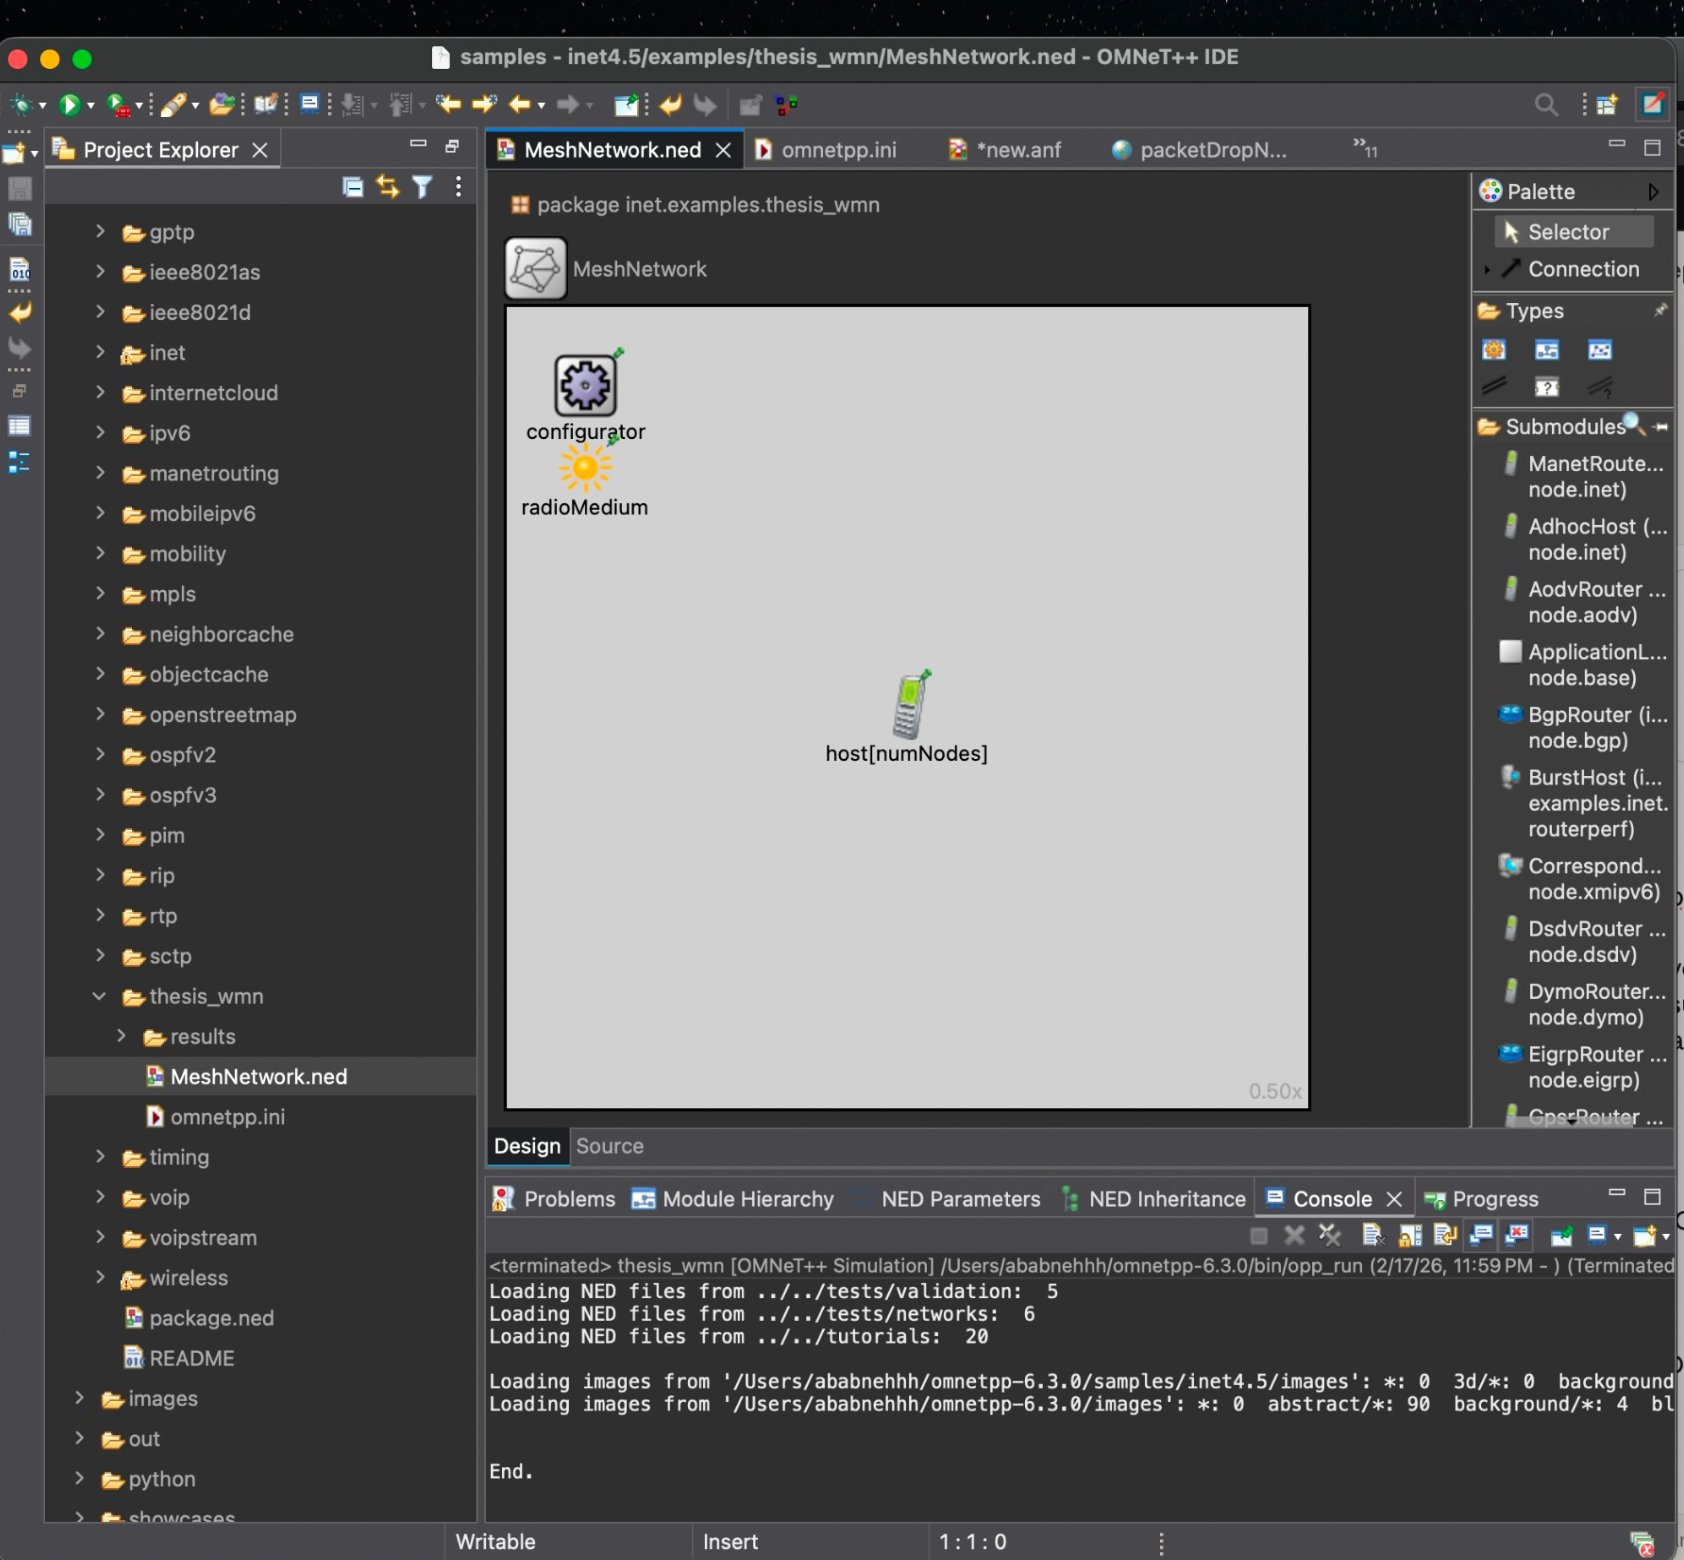
\includegraphics[width=0.95\textwidth]{figures/fig_ned_design}
  \caption{OMNeT++ IDE NED Design view of the \texttt{MeshNetwork} model. The
    submodule palette on the right lists available router types, including
    \texttt{AodvRouter}, \texttt{DsdvRouter}, and \texttt{ManetRouter}. The canvas
    shows the three submodules: \texttt{configurator}, \texttt{radioMedium}, and
    the parameterised \texttt{host[numNodes]} array.}
  \label{fig:ned_design}
\end{figure}

\begin{figure}[ht]
  \centering
  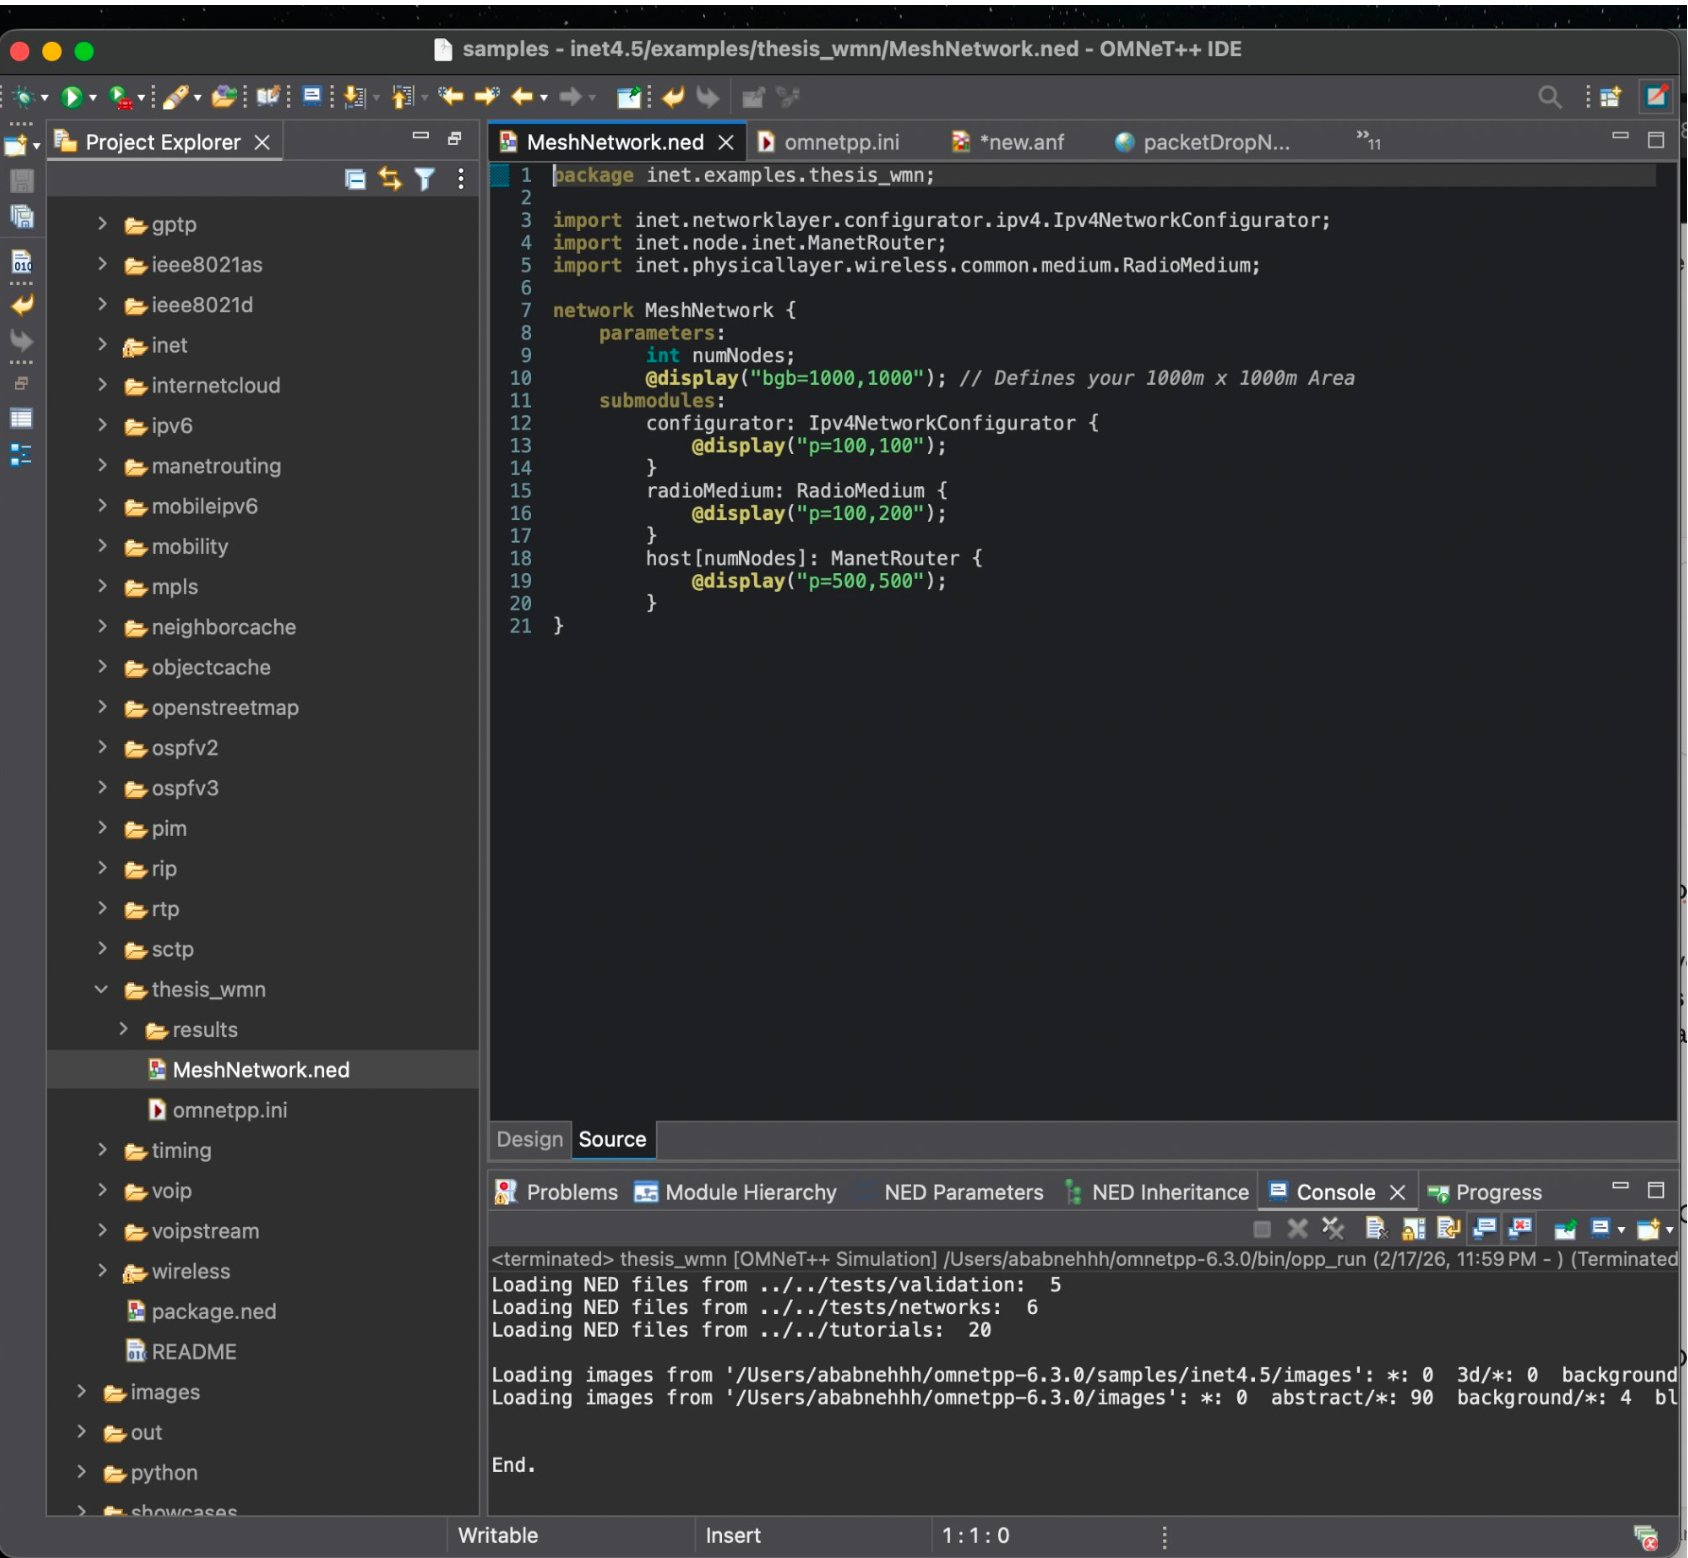
\includegraphics[width=0.95\textwidth]{figures/fig_ned_source}
  \caption{NED source code for \texttt{MeshNetwork} shown in the OMNeT++ IDE Source
    tab. The network imports \texttt{Ipv4NetworkConfigurator}, \texttt{ManetRouter},
    and \texttt{RadioMedium}. Node placement and radio-medium parameters are set in
    \texttt{omnetpp.ini} at runtime.}
  \label{fig:ned_source}
\end{figure}

\begin{figure}[ht]
  \centering
  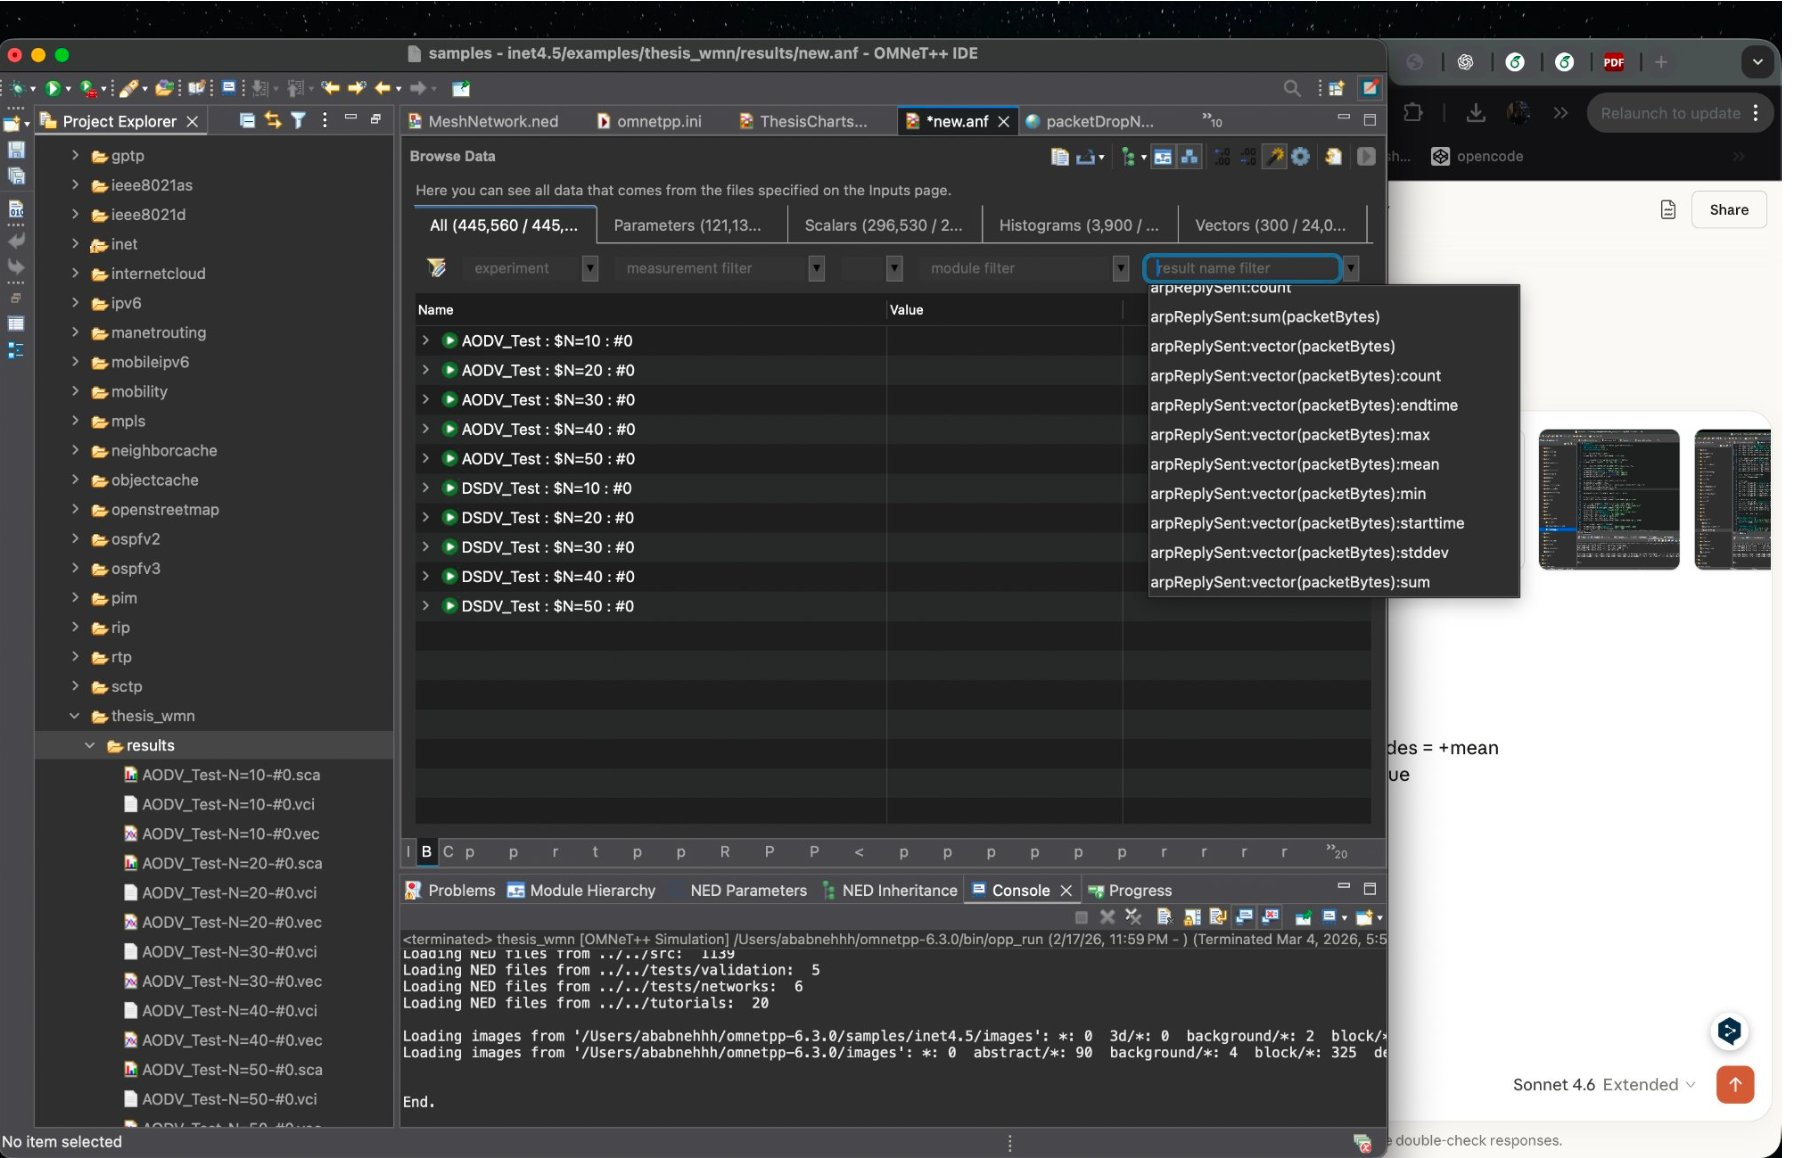
\includegraphics[width=0.95\textwidth]{figures/fig_analysis_tool}
  \caption{OMNeT++ Analysis Tool showing all 10 simulation runs (\texttt{AODV\_Test}
    and \texttt{DSDV\_Test}, each at $N \in \{10, 20, 30, 40, 50\}$). The
    result-name filter panel on the right lists ARP and packet-level statistics
    available for analysis.}
  \label{fig:analysis_tool}
\end{figure}

\section{Network Model}

\subsection{Network Description (NED) File}

The network is defined in \texttt{MeshNetwork.ned}, located in the
\texttt{inet.examples.thesis\_wmn} package. The network contains three submodules:

\begin{itemize}
  \item \texttt{configurator}: An \texttt{Ipv4NetworkConfigurator} instance responsible
    for assigning IPv4 addresses to all nodes. Crucially, \texttt{addStaticRoutes = false}
    is set to prevent the configurator from installing static IP routes that would bypass
    the AODV/DSDV routing logic.
  \item \texttt{radioMedium}: An \texttt{Ieee80211ScalarRadioMedium} instance that
    models propagation, attenuation, and interference using the scalar (single-value per
    channel) model. Background noise is set to $-90$~dBm.
  \item \texttt{host[numNodes]}: An array of \texttt{ManetRouter} instances.
    \texttt{ManetRouter} is a composite module in INET that includes a full TCP/IP stack,
    a WLAN interface, a MANET routing application slot, and an energy storage/consumer
    model.
\end{itemize}

The complete NED file is listed in Appendix~\ref{app:ned}.

\subsection{Node Count Parameterisation}

The number of nodes is swept using OMNeT++'s parameter iteration syntax:

\begin{lstlisting}[caption={Node count sweep in \texttt{omnetpp.ini}.}]
*.numNodes = ${N=10,20,30,40,50}
\end{lstlisting}

This produces 5 separate simulation runs per protocol configuration, for a total of
10~runs.

\section{Node Placement and Spatial Density}

All nodes are placed uniformly at random within a $1000\,\text{m} \times 1000\,\text{m}$
square area. The expected number of neighbours per node (nodes within radio range
$r = 100$~m) follows from the formula for a uniform random point process:

\begin{equation}
  \lambda(N) = (N-1) \cdot \frac{\pi r^2}{A}
  \label{eq:neighbours}
\end{equation}

where $A = 10^6\,\text{m}^2$ is the area and $r = 100$~m is the communication range.
Table~\ref{tab:neighbours} gives the expected neighbour count for each tested $N$.

\begin{table}[ht]
\centering
\caption{Expected number of neighbours per node as a function of network size.}
\label{tab:neighbours}
\begin{tabular}{@{}ccll@{}}
\toprule
$N$ (nodes) & $\lambda$ (expected neighbours) & Network regime & Dominant bottleneck \\
\midrule
10 & 0.28 & Very sparse  & Route availability \\
20 & 0.60 & Sparse       & Route availability / transition \\
30 & 0.91 & Moderate     & Transition \\
40 & 1.22 & Dense        & MAC contention \\
50 & 1.54 & Very dense   & MAC contention \\
\bottomrule
\end{tabular}
\end{table}

At $N = 10$, with fewer than 0.3 expected neighbours per node, the network is near the
connectivity threshold and many source-destination pairs require 4 or more hops. At
$N = 50$, with 1.5 expected neighbours per node, the network is well-connected but the
channel is under heavy load from both data and control traffic.

\section{Mobility Model}

All nodes are stationary for the duration of each simulation run. Stationary behaviour
is implemented using OMNeT++/INET's \texttt{MassMobility} model with
\texttt{speed = 0~mps}. This is functionally equivalent to \texttt{StationaryMobility}
but was chosen to avoid a macOS Qtenv crash that occurs with \texttt{StationaryMobility}
in OMNeT++~6.3 on Apple Silicon when the graphical display is active. The
\texttt{changeInterval} and \texttt{angleDelta} parameters are set to suppress
unassigned parameter warnings:

\begin{lstlisting}[caption={Mobility configuration in \texttt{omnetpp.ini}.}]
**.mobility.typename        = "MassMobility"
**.mobility.initialX        = uniform(0m, 1000m)
**.mobility.initialY        = uniform(0m, 1000m)
**.mobility.initialZ        = 0m
**.mobility.speed           = 0mps
**.mobility.changeInterval  = 1s
**.mobility.angleDelta      = 0deg
**.mobility.initFromDisplayString = false
\end{lstlisting}

The \texttt{initFromDisplayString = false} setting ensures that node positions are
assigned by the \texttt{initialX}/\texttt{initialY} expressions rather than fixed NED
display coordinates, giving a different random placement for each run (determined by the
OMNeT++ random seed).

\section{Radio and MAC Configuration}

The radio interface is configured as IEEE~802.11g in mixed mode with a physical bit rate
of 54~Mbps and a communication range of 100~m. The key radio and MAC parameters are
summarised in Table~\ref{tab:sim_params}.

\begin{table}[ht]
\centering
\caption{Complete simulation parameter reference.}
\label{tab:sim_params}
\small
\begin{tabular}{@{}lll@{}}
\toprule
\textbf{Parameter} & \textbf{Description} & \textbf{Value} \\
\midrule
\multicolumn{3}{@{}l}{\textit{Network topology}} \\
numNodes          & Number of nodes              & \{10, 20, 30, 40, 50\} \\
Area              & Deployment area              & $1000\,\text{m} \times 1000\,\text{m}$ \\
Node placement    & Random uniform               & --- \\
Mobility          & Stationary                   & speed = 0 \\
\midrule
\multicolumn{3}{@{}l}{\textit{Radio / PHY}} \\
Radio medium      & IEEE 802.11 scalar           & \texttt{Ieee80211ScalarRadioMedium} \\
Radio type        & IEEE 802.11 scalar radio     & \texttt{Ieee80211ScalarRadio} \\
Operating mode    & 802.11g mixed                & \texttt{g(mixed)} \\
Bitrate           & Maximum data rate            & 54~Mbps \\
Communication range & Effective radio range      & 100~m \\
Background noise  & Thermal noise floor          & $-90$~dBm \\
\midrule
\multicolumn{3}{@{}l}{\textit{MAC}} \\
MAC type          & Standard DCF                 & \texttt{Ieee80211Mac} \\
CW$_{\min}$       & Minimum contention window    & 31 slots \\
CW$_{\max}$       & Maximum contention window    & 1023 slots \\
Retry limit       & Max retransmissions per frame & 7 \\
\midrule
\multicolumn{3}{@{}l}{\textit{Energy model}} \\
Energy storage    & Ideal (comparative)          & \texttt{IdealEpEnergyStorage} \\
Initial capacity  & Nominal battery size         & 100~J \\
TX power          & Transmitter power            & 1.65~W \\
RX power          & Receiver power               & 1.40~W \\
Sleep power       & Idle/sleep power             & 0.10~W \\
\midrule
\multicolumn{3}{@{}l}{\textit{Traffic}} \\
Application (senders) & UDP constant bit rate    & \texttt{UdpBasicApp} \\
Application (sink)    & UDP sink                 & \texttt{UdpSink} \\
Destination       & Many-to-one                  & \texttt{host[0]} \\
Destination port  & UDP port                     & 5000 \\
Packet size       & Application payload          & 1000~B \\
Send interval     & Randomised inter-packet gap  & \texttt{uniform(0.5s, 1.0s)} \\
Start time        & Randomised start             & \texttt{uniform(1s, 5s)} \\
Stop time         & Traffic cessation            & 49~s \\
\bottomrule
\end{tabular}
\end{table}

\section{Energy Model}

The energy model uses INET's \texttt{StateBasedEpEnergyConsumer} in combination with
\texttt{IdealEpEnergyStorage}. The state-based consumer assigns a fixed power
consumption to each radio state (transmitting, receiving, sleeping), and the ideal
storage integrates consumed power over time to report residual energy capacity.

The \texttt{IdealEpEnergyStorage} module does not model battery chemistry,
self-discharge, or discharge curves; it is a linear integrator. This means the results
are valid for comparative analysis (which protocol consumes more energy) but not for
predicting absolute battery lifetime in deployment. The power levels used (TX:~1.65~W,
RX:~1.40~W, sleep:~0.10~W) are representative of commercial 802.11g radio chipsets such
as the Atheros AR9280.

The key metric recorded is \texttt{residualEnergyCapacity:last} --- the energy remaining
at \texttt{host[25]} (the median node in terms of array index) at the end of each
simulation run. A lower residual capacity indicates higher energy consumption.

\section{Traffic Model}

All nodes except \texttt{host[0]} run a \texttt{UdpBasicApp} that sends 1000~B UDP
datagrams to \texttt{host[0]} (the sink). This many-to-one traffic pattern is
representative of IoT data collection applications (smart meters, environmental sensors,
industrial monitors) where all field devices report to a central gateway or server.

Sending is randomised in two ways:
\begin{itemize}
  \item \textbf{Inter-packet interval:} drawn uniformly from $[0.5\,\text{s}, 1.0\,\text{s}]$
    to prevent synchronisation effects where all nodes transmit in lock-step.
  \item \textbf{Start time:} drawn uniformly from $[1\,\text{s}, 5\,\text{s}]$ to stagger
    initial transmissions and avoid a startup burst.
\end{itemize}

Traffic stops at 49~s, leaving 1~s for the last in-flight packets to arrive before the
simulation ends at 50~s.

\section{Performance Metrics and Recording}

Five metrics are recorded:

\begin{enumerate}
  \item \textbf{Total bytes received} (\texttt{packetReceived:sum(packetBytes)}) at
    \texttt{host[0]}, in bytes. This is the primary throughput indicator.
  \item \textbf{Packet reception count} (\texttt{packetReceived:count}) at
    \texttt{host[0]}, the number of successfully delivered application packets.
  \item \textbf{End-to-end delay} (\texttt{endToEndDelay:mean} recorded as a scalar at
    the \texttt{UdpSink} module).
  \item \textbf{Residual energy capacity} (\texttt{residualEnergyCapacity:last}) at
    \texttt{host[25]}, in joules.
  \item \textbf{Packet drop count} (\texttt{packetDropped[noRouteFound]:count}) at all
    nodes, summed across the network.
\end{enumerate}

OMNeT++ result files (\texttt{.sca} for scalars, \texttt{.vec} for time series) are
written to the \texttt{results/} subdirectory and analysed using the built-in OMNeT++
Analysis Tool and the Python \texttt{omnetpp.scave} interface.

\section{Simulation Configurations}

Two named simulation configurations are defined in \texttt{omnetpp.ini}:

\begin{lstlisting}[caption={AODV and DSDV configuration sections in \texttt{omnetpp.ini}.}]
[Config AODV_Test]
description = "Simulate Reactive AODV"
**.routingApp.typename = "Aodv"

[Config DSDV_Test]
description = "Simulate Proactive DSDV"
**.routing.typename = "Dsdv"
\end{lstlisting}

The difference in parameter path (\texttt{routingApp} for AODV vs.\ \texttt{routing}
for DSDV) reflects the INET module hierarchy: AODV is implemented as an
application-layer routing process (\texttt{AodvRouting} module inside
\texttt{ManetRouter}), while DSDV is implemented at the network layer
(\texttt{DsdvRouting} module). Both interact with the same IP forwarding table and WLAN
interface stack.
